% !TEX root = ../../lectures.tex
\section{Where do Alfv\'en waves come from in the Milky Way?}
\subsection{Large–scale driving and the turbulence cascade}

Magnetized turbulence in the Galactic interstellar medium (ISM) is continually stirred on large scales by energetic processes (e.g.\ clustered supernovae, expanding superbubbles, Galactic shear). Whatever the detailed mechanism, the key point is that energy is \emph{injected} into the plasma at some outer scale \(L \sim 10 \)~pc with a characteristic velocity fluctuation \(u_L\). From there, nonlinear interactions transfer this energy to progressively smaller eddies and wave packets. This scale-to-scale transfer is the \emph{cascade}. 

Between the outer (forcing) scale \(L\) and the microscopic \emph{dissipation} scale \(\ell_{\rm d}\) (where viscosity, resistivity, or kinetic effects finally convert turbulent energy into heat), the dynamics are dominated by nonlinear advection and are largely insensitive to the details of forcing or dissipation. This interval of scales \( \ell_{\rm d} \ll \ell \ll L \) is the \emph{inertial range}. Statistics in this range are expected to be \emph{universal}, set primarily by the mean energy flux \(\varepsilon\) cascading through scales (energy per unit mass per unit time).

\paragraph{Kolmogorov’s dimensional argument (hydrodynamic baseline).}
Kolmogorov (1941) reasoned that, in the inertial range, the only relevant quantities for an eddy of size \(\ell\) are its velocity amplitude \(u_\ell\) and the constant energy flux \(\varepsilon\). Dimensional analysis gives
\[
\varepsilon \sim \frac{u_\ell^2}{\tau_\ell}\sim \frac{u_\ell^3}{\ell}
\quad\rightarrow\quad
u_\ell \sim (\varepsilon\,\ell)^{1/3},\quad 
\tau_\ell \sim \frac{\ell}{u_\ell} \sim \varepsilon^{-1/3}\,\ell^{2/3}.
\]
Defining the one-dimensional energy spectrum \(E(k)\) by
\[
\frac{1}{2}\langle u^2\rangle \;=\; \int_0^\infty E(k)\,{\rm d}k,
\]
and using the correspondence \(\ell\sim k^{-1}\), the velocity at scale \(k\) scales as \(u_k^2\sim k\,E(k)\). 
%
Substituting \(u_k\sim (\varepsilon k^{-1})^{1/3}\) gives the celebrated inertial-range spectrum
\begin{remark}
\[
E(k)\;=\; C_K\,\varepsilon^{2/3}\,k^{-5/3}
\]
\end{remark}
with \(C_K\) an order-unity constant. The essence is: a constant energy flux \(\varepsilon\) through scales, an eddy turnover time \(\tau_\ell\sim\ell/u_\ell\), and no dependence on forcing or dissipation details.

This is called \emph{Kolmogorov spectrum law or the -5/3 law}. 

\begin{figure}[t] 
\centering 
%\includegraphics[width=0.90\textwidth]{figures/richardson.pdf} 
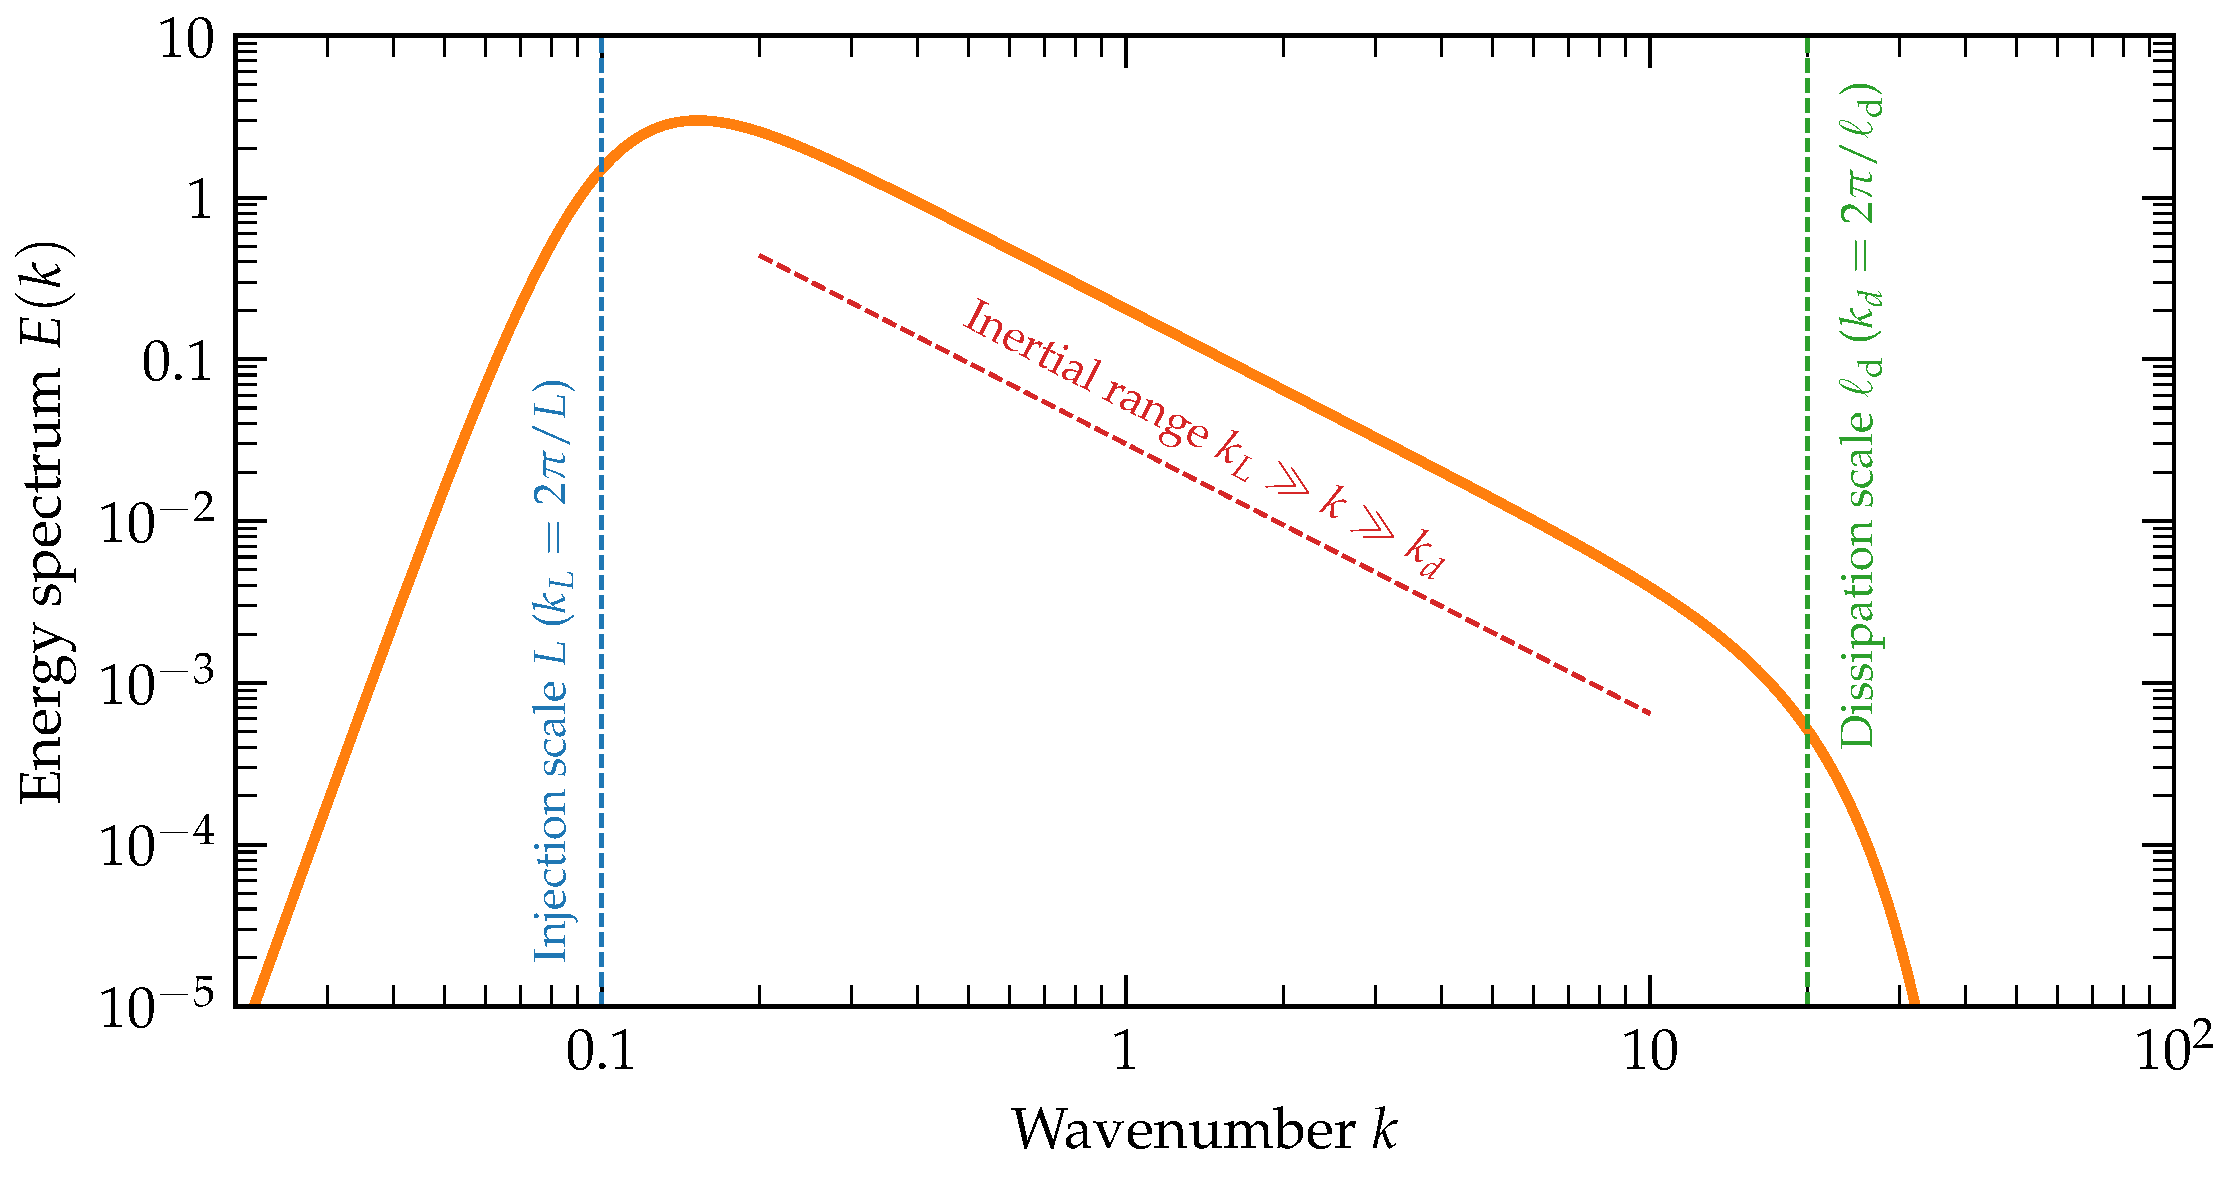
\includegraphics[width=0.99\textwidth]{figures/kolmogorov_cascade_schematic.pdf} 
\caption{.} 
\label{fig:kolmorogov} 
\end{figure}

%Richardson (1922) introduced the energy cascade concept as: “Big whorls have little whorls that feed on their velocity; And little whorls have lesser and so on to viscosity.”

{\color{red}Dire che la turbolenza viene dalle equazione di Navier-Stokes.}

\begin{figure}[t] 
\centering 
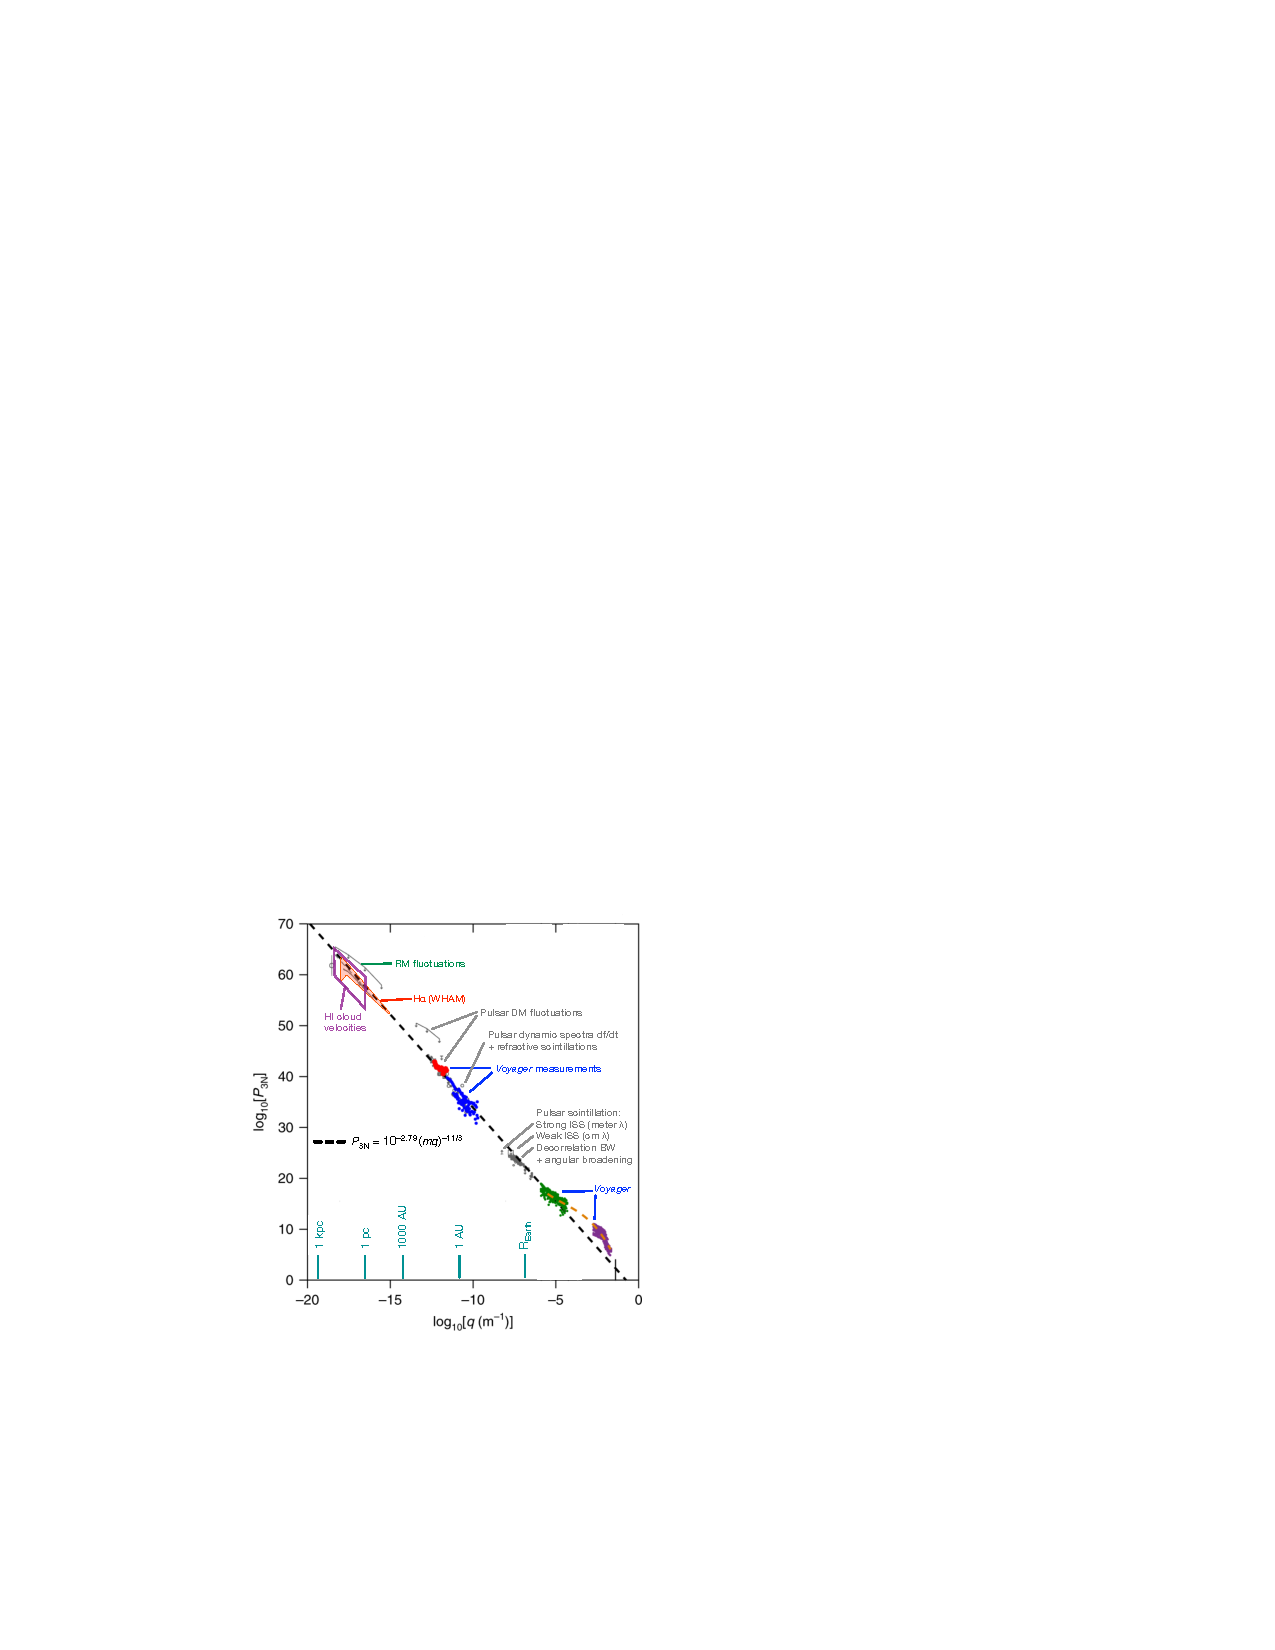
\includegraphics[width=0.7\textwidth]{figures/ism_turbulence.pdf}
\caption{Big Power Law in the sky: electron density power spectrum in the ISM  (Armstrong et al. ApJ 433, 209, 1995) Radio Scintillations measure power
density spectrum in local ISM.. Power law spans 12 decades in
wavenumber space.
Outer
scale
Exhibits a k Kolmogorov-like
spectrum.Power-law in the sky. Armstrong, Nature '81 Spangler '95. ?} 
\label{fig:ismturbulence} 
\end{figure}

\paragraph{From hydrodynamics to MHD: Alfv\'enic cascades.}
In a magnetized plasma the turbulence can be decomposed into Alfvénic and compressive (magnetosonic) parts. The Alfvénic component---incompressible, transverse perturbations tied to the mean magnetic field \(\mathbf B_0\)---dominates much of the ISM cascade. Nonlinear interactions transfer energy mainly by \emph{distorting} counter-propagating Alfvén wave packets. 

Two classic consequences follow:
\begin{itemize}
  \item The cascade is \emph{anisotropic}: eddies become increasingly elongated along \(\mathbf B_0\). In modern language (Goldreich–Sridhar), \emph{critical balance} relates the linear Alfvén time \( (k_\parallel v_A)^{-1} \) to the nonlinear time \( (k_\perp u_{k_\perp})^{-1} \), producing a Kolmogorov-like spectrum \emph{in the perpendicular direction}, \(E(k_\perp)\propto \varepsilon^{2/3}k_\perp^{-5/3}\).
  \item Magnetic and kinetic energies tend toward near-equipartition within the Alfvénic cascade, so the same scaling applies (up to constants) to \(\delta\mathbf v\) and \(\delta\mathbf B\) fluctuations.
\end{itemize}
Older phenomenology (Iroshnikov–Kraichnan) predicts a slightly shallower slope \(k^{-3/2}\) owing to weakened interactions; observations and simulations in many astrophysical settings favor a Kolmogorov-like \(-5/3\) spectrum in \(k_\perp\), with anisotropy set by the mean field strength.

\paragraph{What the inertial range means physically.}
\begin{itemize}
  \item \textbf{Universality:} statistics at \(\ell\) depend only on \(\varepsilon\) (and, in MHD, on the direction relative to \(\mathbf B_0\)), not on how the turbulence was stirred or how it will ultimately dissipate.
  \item \textbf{Self-similar cascade:} energy injected near \(L\) passes through a hierarchy of eddies/wave packets with turnover time \(\tau_\ell\propto \ell^{2/3}\) until it reaches \(\ell_{\rm d}\), where microphysics takes over.
  \item \textbf{Spectral signature:} a power-law energy spectrum—\(E(k)\propto k^{-5/3}\) for hydrodynamic turbulence; in MHD, the same \(-5/3\) scaling appears in the \emph{perpendicular} spectrum of Alfvénic turbulence, with anisotropy \(k_\parallel \ll k_\perp\) that strengthens toward small scales.
\end{itemize}

\paragraph{Takeaway for the Milky Way.}
Large-scale Galactic driving maintains a steady energy flux \(\varepsilon\) into the ISM. In the inertial range, that flux feeds an anisotropic Alfvénic cascade with a Kolmogorov-like perpendicular spectrum. The resulting sea of broadband Alfvénic fluctuations is the natural reservoir of ``where Alfvén waves come from’’ in the Galaxy: they are not produced one frequency at a time, but emerge continuously from the nonlinear cascade that carries energy from \(L\) down to the dissipation scale.

\begin{remark}{Turbulent energy and timescales in the ISM.}

Observations and theory indicate that the Galactic ISM is stirred on large scales by superbubbles and clustered supernovae~\ref{2004Ap&SS.289..323M}. A typical baseline is an outer (forcing) scale \(L\equiv l_0\simeq 100~\mathrm{pc}\) with a characteristic velocity comparable to the sound speed of the warm phases,
\(u_0\sim c_s\simeq 10~\mathrm{km\,s^{-1}}\).

In a Kolmogorov‐type cascade the flow sheds energy at roughly one eddy per scale, so the global decay time of turbulence is set by the turnover time of the largest eddies,
\[
\tau_0 \sim \frac{l_0}{u_0}
\;\simeq\; 10^{7}~\mathrm{yr}.
\]
Thus, even if microscopic dissipation is weak, sustained turbulence requires continuous driving on $\sim$Myr timescales.

The corresponding (mass‐specific) energy flux through scales is
\(\varepsilon \sim u_0^{3}/l_0\),
so the \emph{volumetric} turbulent dissipation rate is
\[
\epsilon_{\rm turb} \sim \rho\,\frac{u_0^{3}}{l_0}.
\]
Adopting a representative warm–ISM density \(n\simeq 1~\mathrm{cm^{-3}}\) and
\(\rho\simeq 1.4\,m_p n \approx 2.3\times10^{-24}~\mathrm{g\,cm^{-3}}\),
one obtains
\[
\epsilon_{\rm turb}\;\approx\; 8\times10^{-27}\ \mathrm{erg\,cm^{-3}\,s^{-1}}.
\]

To compare with the available power from supernovae, distribute the SN mechanical luminosity over the star–forming disc volume
\(V\simeq 2\pi h R_d^2\),
with scale height \(h\simeq 100~\mathrm{pc}\) and radius \(R_d\simeq 10~\mathrm{kpc}\).
Using \(E_{\rm SN}=10^{51}~\mathrm{erg}\) and a Galactic rate
\(\mathcal R_{\rm SN}\simeq 1/50~\mathrm{yr^{-1}}\),
\[
\epsilon_{\rm SN}
=\frac{E_{\rm SN}\,\mathcal R_{\rm SN}}{2\pi h R_d^2}
\;\approx\;
3.4\times10^{-25}\ \mathrm{erg\,cm^{-3}\,s^{-1}}.
\]

Is there enough power to maintain the cascade?
The ratio
\(
\tfrac{\epsilon_{\rm turb}}{\epsilon_{\rm SN}} \approx 0.02
\)
shows that only a \(\sim\!2\text{–}3\%\) coupling of SN mechanical energy into turbulent motions is sufficient—comfortably plausible given other sinks (radiation, cosmic rays, winds). In short, with \(L\sim100\ \mathrm{pc}\) and \(u_0\sim10\ \mathrm{km\,s^{-1}}\), the ISM would decay its turbulence in \(\sim10\) Myr unless it is continuously powered, and ordinary supernova activity can readily supply the needed \(\sim10^{-26} \, \mathrm{erg\,cm^{-3}\,s^{-1}}\).
\end{remark}

\subsection{Self–generated Alfv\'en waves: Kulsrud’s argument}

Cosmic rays (CRs) move individually at \(v\simeq c\), but on average they drift a little along the large–scale magnetic field \(\mathbf B_0\) with bulk speed \(v_D\) set by their
pressure gradient. If \(v_D>v_A\), the CR pitch–angle distribution acquires a small anisotropy that resonantly excites forward–propagating Alfv\'en waves. Those waves
scatter the CRs in pitch angle until, in the wave frame, the distribution becomes nearly isotropic. During this relaxation the CRs lose \emph{parallel} momentum to the
waves/plasma, and their bulk drift is reduced from \(v_D\) toward \(v_A\). Thus super–Alfv\'enic CR streaming \emph{self–generates} the very Alfv\'enic turbulence
that ultimately limits the streaming speed.

\paragraph{Momentum bookkeeping (step by step).}

Kulsrud’s argument captures the transfer of energy from cosmic rays to Alfv\'en waves without needing the detailed wave–particle kinetics.

Let \(P_{\rm cr}\) denote the cosmic ray parallel momentum density before the isotropization when they stream with a drift velocity \( v_D \)
%
\[
P_{\rm cr}^{\rm before} = n(>p) m_p \gamma v_D
\]
after isotropization in the wave frame, they have (in the Galaxy frame) a net velocity of \(v_A\), then their momentum is
\[
P_{\rm cr}^{\rm after} = n(>p) m_p \gamma v_A
\]

We use the fact that only CRs near the \emph{gyroresonant} momentum
\(p_{\rm res}=Ze\,B_0/(k\,c)\) efficiently exchange momentum with waves at wavenumber
\(k\). 

i.e.\ number density of CRs above the resonant momentum

Then this process implies a parallel momentum change of the order of
%
\[
dP_{\rm cr} = n(>p) m_p \gamma (v_A - v_D) < 0
\]

We remind that pitch–angle scattering with diffusion coefficient \(D_{\mu\mu}\) isotropizes
the distribution at a rate
\[
\nu_s \;\equiv\; \tau^{-1} \;\sim\; D_{\mu\mu}
\quad\rightarrow\quad
\frac{dP_{\rm cr}}{dt}\;\simeq\; -\nu_s\,n(>p) m_p \gamma (v_D - v_A)
\]

This is just “momentum lost per isotropization time.’’

By momentum conservation the waves gain the same parallel momentum:
\[
\frac{dP_{w}}{dt}\;=-\frac{dP_{\rm cr}}{dt}
\]
For a (linear) Alfv\'en wave, the \emph{wave momentum density} and \emph{magnetic energy
density} are related by
\[
P_{w} \;=\; \frac{E_{\rm tot}}{v_A} \;=\; \frac{2W}{v_A},
\qquad
W \equiv \frac{\delta B^2}{8\pi},
\]
because magnetic and kinetic energies are equal on average
(\(E_{\rm tot}=2W\)) and the Alfv\'en Poynting flux is \(S=v_A E_{\rm tot}\).
Therefore
\[
\frac{dW}{dt}\;=\;\frac{v_A}{2}\,\nu_s\,n(>p) m_p \gamma (v_D - v_A)~.
\]
This already gives the \emph{power per unit volume} that goes into waves.

At resonance, quasi–linear theory gives
\[
\nu_s \;\sim\; D_{\mu\mu}(k)
\;\propto\; \Omega\,\left(\frac{\delta B_k}{B_0}\right)^{\!2},
\]
with \(\Omega=eB_0/(m_pc)\) for protons, and \(\delta B_k\) the wave amplitude around
wavenumber \(k\). 

\[
\frac{dW_k}{dt}\;\propto\;
v_A\,\Omega\,
\left(\frac{\delta B_k}{B_0}\right)^{\!2}\;
n_{\rm cr}(>p_{\rm res})\;\frac{p_{\rm res}}{c}\;
\bigl(v_D - v_A\bigr).
\]

Writing the growth in the standard linear form
\(\partial_t W_k = 2\,\Gamma_w(k)\,W_k\) with \(W_k\propto \delta B_k^2\) immediately
yields
\begin{remark}
\[
\Gamma_w(k)\;\propto\;\Omega\,
\frac{n_{\rm cr}(>p_{\rm res})}{n_i}\,
\Bigl(\frac{v_D}{v_A}-1\Bigr)\,~.
\]
\end{remark}

\paragraph{ISM scale estimate.}
Take a warm–ISM reference point: \(B_0=5~\mu\mathrm G\),
\(n_i\simeq 1~\mathrm{cm^{-3}}\Rightarrow \Omega_p\simeq 0.05~\mathrm{s^{-1}}\).
For resonant CRs near a few GeV, a typical integrated density is
\(n_{\rm cr}(>p_{\rm res})\sim 10^{-10}~\mathrm{cm^{-3}}\).
If streaming is moderately super–Alfv\'enic, say \(v_D\simeq 2v_A\), then
\[
\gamma \;\sim\;
\frac{\pi}{4}\,(0.05~\mathrm{s^{-1}})
\left(\frac{10^{-10}}{1}\right)(1)
\;\approx\; 4\times10^{-12}~\mathrm{s^{-1}}
\;\approx\; 1.3\times10^{-4}~\mathrm{yr^{-1}}.
\]
The corresponding growth time, \( \gamma^{-1}\sim 8\times 10^{3}~\mathrm{yr}\),
is orders of magnitude shorter than CR residence times in the Galaxy, so in regions
where damping is not overwhelming the CRs can indeed \emph{self–generate} the
Alfv\'enic turbulence that regulates their own drift to \(v_A\).

\paragraph{Takeaway.}
Super–Alfv\'enic CR streaming is unstable. Resonant wave growth taps the CR pressure
gradient until pitch–angle scattering reduces the drift to \(v_A\). The steady wave
amplitude at each \(k\) is set by the balance \(\gamma(k)=\Gamma_{\rm damp}(k)\); the
resulting spectrum governs the scattering rate and thus the CR transport.

\paragraph{What sets the amplitude in the ISM.}
In different phases of the ISM the relevant damping can be ion–neutral friction, non-linear Landau damping, turbulent damping by the ambient cascade, or simple collisional/resistive losses.
Balancing $\gamma(k)$ against the dominant $\Gamma_{\rm damp}(k)$ fixes $\delta B(k)$ (via $W=\delta B^2/8\pi$) and thus the local scattering rate $D_{\mu\mu}(p)$ and parallel diffusion coefficient $\kappa_\parallel(p)$—closing the loop between CR transport and their self-generated turbulence.


